% !TeX spellcheck = en_US
% -*-coding: utf-8 -*-

%% Ejemplo
%% -------

\section{Ejemplo}
\label{sec:ejemplo}

Esta sección presenta un ejemplo de un pequeño lenguaje para ilustrar los conceptos de MDLE.

DSL(\textit{Oficinas y Empleados}): El siguiente lenguaje proporciona conceptos para definir
las oficinas  y empleados, así como las relaciones entre los empleados en el modelo que dos o 
más de ellos trabajan juntos. 

\itemize{
 \item {Descargue e instale EMFText a través del gestor de actualizaciones de Eclipse utilizando el enlace: \textit{http://emftext.org/update}} 
  seleccione \textit{EMFText}. También seleccione utlizando el enlace:\textit{http://download.eclipse.org/releases/juno/201209280900}
  \textit{Modeling} - \textit{Ecore Tools SDK}, este permitira herramientas a los modelos basados en diagramas.
 \item {Crear un nuevo proyecto y una carpeta llamada \textit{metamodel}. donde se añadiran 
 las clases para el desarrollo del lenguaje.}
 \item{Crear un nuevo \textit{Ecore Diagram} para la creación del Metamodelo (Sintaxis Abstracta)}.
 \begin{figure}[h]
 \begin{center}
 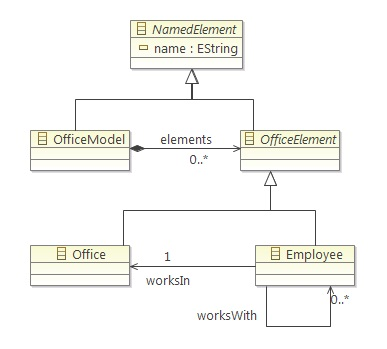
\includegraphics[width=0.7\textwidth] 
 {img/Metamodelo.jpg}
 \caption{Metamodelo \textit{Office}} \label{}
 \end{center}
 \end{figure}
 \item{Crear un nuevo \textit{EMF Model} y seleccione \textit{Ecoremodel}} esto creara un archivo con extensión \textit{.genmodel}
  que contiene información adicional para el \textit{codegenerartion}. También es considerado una vista alterna del \textit{Metamodelo}. 
 \begin{figure}[h]
 \begin{center}
 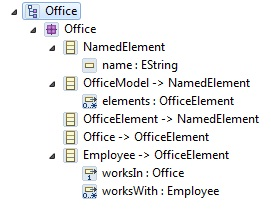
\includegraphics[width=0.7\textwidth] 
 {img/MetamodeloGenmodel.jpg}
 \caption{Metamodelo.Genmodel \textit{Office}} \label{}
 \end{center}
 \end{figure}
 \item{Crear la sintaxis conreta. Para el desarrollo de este se tiene dos opciones: (1)Generar la sintaxis automaticamente por medio del archivo con extensión \textit{.genmodel}.
 click derecho sobre el archivo y se elige la opción \textit{Generate HUTN Sintax}. 
 (2)Crear un nuevo archivo con extensión \textit{.cs} donde se especificara paso a paso la sintaxis.
 }
 }
                                               